%
% section 2.2
%
\section{Η Πρόσβαση στο Μέσο}

Σε ένα δίκτυο, το μέσο μεταφοράς (καλώδιο, οπτική ίνα κλπ) είναι κοινό για όλους τους υπολογιστές που συνδέονται σε αυτό. Προκειμένου να εξασφαλιστεί η ομαλή μετάδοση των δεδομένων, θα πρέπει κάθε φορά να μεταδίδει μόνο ένας υπολογιστής. Αν δυο υπολογιστές αποκτήσουν ταυτόχρονα πρόσβαση για μετάδοση στο μέσο, τα πακέτα τους θα συγκρουστούν με αποτέλεσμα την καταστροφή τους. Καμιά από τις δύο μεταδόσεις δεν θα φτάσει στο προορισμό της. Για να έχουμε επιτυχή μετάδοση πρέπει να τηρούνται οι παρακάτω προϋποθέσεις:\\

\begin{itemize}
\item Εισαγωγή των δεδομένων στο μέσο μετάδοσης χωρίς να υπάρχει σύγκρουση με άλλα δεδομένα.
\item Ο παραλήπτης να λάβει τα δεδομένα γνωρίζοντας ότι αυτά δεν έχουν καταστραφεί σε σύγκρουση δεδομένων (data collision) κατά τη μετάδοση.
\end{itemize}

Για να επιτευχθούν τα παραπάνω, σε κάθε δίκτυο υπάρχει μια σειρά από κανόνες με βάση τους οποίους γίνεται η εισαγωγή των δεδομένων στο μέσο μετάδοσης. Οι κανόνες αυτοί αποτελούν τη \emph{μέθοδο προσπέλασης (access method)}. Είναι σημαντικό οι κανόνες αυτοί να είναι κοινοί για όλους τους υπολογιστές ενός συγκεκριμένου δικτύου. Αν κάποιοι υπολογιστές χρησιμοποιούν διαφορετικούς, το δίκτυο θα αποτύχει γιατί κάποιες μέθοδοι προσπέλασης θα κυριαρχήσουν στο καλώδιο. Σε γενικές γραμμές σκοπός των μεθόδων προσπέλασης είναι να εμποδίσουν την ταυτόχρονη εισαγωγή δεδομένων στο μέσο πρόσβασης. Εξασφαλίζοντας ότι μόνο ένας υπολογιστής μεταδίδει δεδομένα κάθε φορά, οι μέθοδοι προσπέλασης κρατούν οργανωμένες τις διαδικασίες αποστολής και λήψης δεδομένων δικτύου.

Υπάρχουν γενικά τρεις τρόποι για την αποφυγή ταυτόχρονης χρήσης του μέσου μετάδοσης:

\begin{itemize}
\item Μέθοδοι \textbf{Carrier Sense Multiple Access, CSMA} (Πολλαπλής πρόσβασης με ακρόαση φέροντος)
  \begin{itemize}
    \item Με \textbf{Ανίχνευση Σύγκρουσης} (Collision Detection), CSMA/CD
    \item Με \textbf{Αποφυγή Σύγκρουσης} (Collision Avoidance), CSMA/CA
  \end{itemize}
\item Μέθοδος με \textbf{Κουπόνι Διέλευσης} (Token Passing) που δίνει δυνατότητα μεμονωμένης αποστολής δεδομένων
\item Μέθοδος \textbf{Απαίτησης Προτεραιότητας}
\end{itemize}

\begin{inthebox}
\textbf{Τι είναι το CSMA και το CSMA/CD; (εκτός εξεταστέας ύλης)}

Η τεχνική πολλαπλής πρόσβασης με ανίχνευση φέροντος ουσιαστικά σημαίνει ότι πριν αρχίσει η μετάδοση, γίνεται πρώτα ανίχνευση της γραμμής για να διαπιστωθεί αν γίνεται ήδη μετάδοση από κάποιο άλλο υπολογιστή. Το ``φέρον'' είναι ένα σήμα που υπάρχει στη γραμμή όσο γίνεται οποιαδήποτε μετάδοση. Δεν είναι απαραίτητο για τον υπολογιστή που επιθυμεί να μεταδώσει να προσπαθήσει να διαβάσει τα δεδομένα της γραμμής για να διαπιστώσει αν είναι σε χρήση. Η ανίχνευση του φέροντος είναι μια σχετικά απλή διαδικασία που μπορεί να γίνει ήδη από τα κυκλώματα της κάρτας δικτύου.

Ο υπολογιστής που πρόκειται να μεταδώσει, αν διαπιστώσει την ύπαρξη φέροντος θα περιμένει μέχρι το τέλος της μετάδοσης για να ξεκινήσει. Προσέξτε ότι έτσι αποφεύγεται μόνο το ένα είδος σύγκρουσης!

Αν έχουμε δύο υπολογιστές σε αναμονή για μετάδοση, είναι πιθανόν να ξεκινήσουν και οι δυο ταυτόχρονα με το που θα ελευθερωθεί η γραμμή. Στην περίπτωση αυτή θα έχουμε πάλι σύγκρουση. Εδώ μπορεί να αναλάβει η Ανίχνευση Σύγκρουσης (Collision Detection).  Και σε αυτήν την περίπτωση, ένα κύκλωμα στην κάρτα δικτύου μπορεί να αντιληφθεί ότι στη γραμμή γίνονται παραπάνω από μια μεταδόσεις (άρα έχουμε σύγκρουση). Ένας απλός τρόπος βασίζεται στο γεγονός ότι η ισχύς του σήματος στη γραμμή είναι μεγαλύτερη με δύο μεταδόσεις από ότι με μια. Έτσι γνωρίζουμε ότι τα δεδομένα καταστράφηκαν και σταματάμε τη μετάδοση, κερδίζοντας χρόνο.

\textbf{Τι είναι το Κουπόνι Διέλευσης;}

Είναι ένας διαφορετικός τρόπος να σκεφτούμε την πολλαπλή πρόσβαση: Μέσα στο δίκτυο κυκλοφορεί, από κόμβο σε κόμβο, ένα ειδικό πακέτο (κουπόνι) το οποίο χρησιμοποιείται ως φορέας μεταφοράς δεδομένων. Ο κόμβος που επιθυμεί να μεταδώσει, θα αποσύρει το κουπόνι από το δίκτυο, θα βάλει σε αυτό τα δεδομένα του και θα το ξαναστείλει. Ο παραλήπτης θα πάρει το κουπόνι, θα διαβάσει τα δεδομένα και θα το αφήσει ξανά ``άδειο'' στο δίκτυο. Το κουπόνι μπορεί έπειτα να το πάρει άλλος κόμβος κ.ο.κ.\\
\end{inthebox}

\subsection*{Πρότυπα Τοπικών Δικτύων}

Οι σημαντικότερες τοπολογίες τοπικών δικτύων καθώς και τα πρωτόκολλα που θα χρησιμοποιούνταν από τους σταθμούς εργασίας, αναπτύχθηκαν αρχικά από διάφορες εταιρείες. Ωστόσο διαφορετικοί κατασκευαστές χρησιμοποιούσαν διαφορετικά, δικά του ο καθένας, πρωτόκολλα με αποτέλεσμα να μην είναι συνήθως δυνατή η επικοινωνία υπολογιστών διαφορετικών κατασκευαστών. Η αρχή της τυποποίησης έγινε όταν το \emph{Ινστιτούτο Ηλεκτρολόγων και Ηλεκτρονικών Μηχανικών} (IEEE, Institute of Electrical and Electronic Engineers, IEEE) και η \emph{Ευρωπαϊκή Ένωση Κατασκευαστών Υπολογιστών} (European Computer Manufacturing Association, ECMA) συμφώνησαν να ακολουθήσουν το πρότυπο OSI. 

Στο OSI, η ανταλλαγή μηνυμάτων και η επικοινωνία των σταθμών εργασίας αναλύεται σε επτά επίπεδα. Τα δύο κατώτερα είναι το \emph{επίπεδο σύνδεσης δεδομένων} και το \emph{φυσικό επίπεδο}. Σε αυτά καθορίζεται ο τύπος του δικτύου και το πρωτόκολλο επικοινωνίας. Η υλοποίηση των δύο επιπέδων γίνεται με συνδυασμό υλικού και λογισμικού.

Για την δημιουργία του προτύπου, το IEEE δημιούργησε μια επιτροπή γνωστή ως 802 με έργο τον καθορισμό προτύπων για τα τοπικά (LAN) και τα μητροπολιτικά (ΜΑΝ) δίκτυα. 

\begin{inthebox}
\textbf{Τι είναι τα Μητροπολιτικά Δίκτυα; (Metropolitan Area Network, MAN)}

Τα μητροπολιτικά δίκτυα καλύπτουν αποστάσεις και γεωγραφικές περιοχές μεγαλύτερες από τα τοπικά δίκτυα αλλά γενικά μικρότερες από αυτές που καλύπτει ένα δίκτυο ευρείας περιοχής. Ένα τοπικό δίκτυο καλύπτει συνήθως τις ανάγκες ενός κτηρίου ή συμπλέγματος κτηρίων, ενώ ένα ευρείας περιοχής μπορεί να ενώνει μεταξύ τους πόλεις ή ακόμα και ηπείρους. Ένα μητροπολιτικό δίκτυο συνήθως έχει μέγεθος τέτοιο ώστε να καλύπτει μια πόλη.\\
\end{inthebox}

\begin{figure}[!ht]
  \centering
  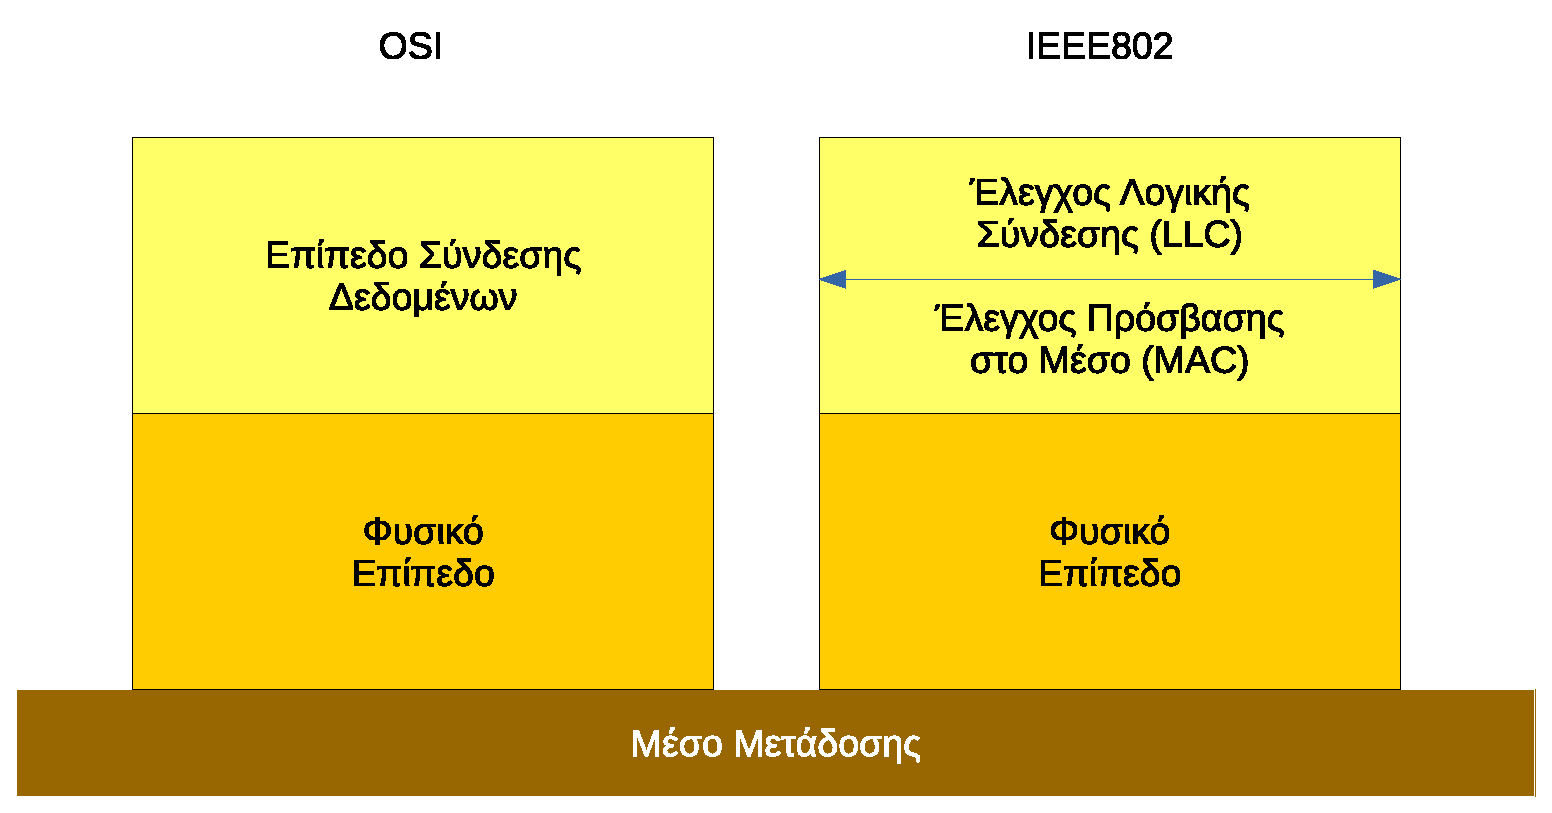
\includegraphics[width=0.95\textwidth]{images/chapter2/2-2}
  \caption {\textsl{Σχέση Μοντέλων Αναφοράς OSI και IEEE802}}
  \label{2-2}
\end{figure}

Η επιτροπή 802 χωρίσθηκε σε έξι (6) μικρότερες υποεπιτροπές. Κάθε μια από αυτές ασχολήθηκε με την ανάπτυξη επιμέρους προτύπων για τους διαφορετικούς τύπους δικτύων. Αργότερα δημιουργήθηκαν ακόμα περισσότερες υποεπιτροπές (π.χ. για τα πρότυπα των ασύρματων δικτύων). Τα αποτελέσματα κάθε υποεπιτροπής είναι γνωστά με την ονομασία IEEE 802.x όπου x ο αριθμός της υποεπιτροπής. Για παράδειγμα, η υποεπιτροπή 3 σχεδίασε το πρότυπο IEEE 802.3 στο οποίο βασίζεται το Ethernet που θα εξετάσουμε σε επόμενη ενότητα.

Με βάση το έργο της επιτροπής 802, το δεύτερο επίπεδο του OSI χωρίσθηκε σε δύο υπο-επίπεδα (σχήμα \ref{2-2}): το υπο-επίπεδο \emph{Ελέγχου Λογικής Σύνδεσης της Γραμμής} (Logical Line Control, LLC) που περιγράφεται στο IEEE802.2 και το υπο-επίπεδο \emph{Ελέγχου Πρόσβασης στο Μέσο} (Media Access Control, MAC) που περιγράφεται στα IEEE 802.3, ΙΕΕΕ 802.4 και ΙΕΕΕ 802.5.

